\documentclass{beamer}
\usepackage{listings}
\usepackage{tikz}
\usetikzlibrary{shapes.geometric, arrows, positioning}
\usetheme{metropolis}
\title{Maintaining Botania for Forge and Fabric}
\date{June 11, 2022}
\author{williewillus}
\institute{Violet Moon Modding}
\titlegraphic{
\includegraphics{../../web/assets/img/logo.png}}

\tikzstyle{std} = [rectangle, minimum width=1cm, minimum height=0.7cm, text centered, draw=black, fill=blue!10]
\tikzstyle{arrow} = [thick,->,>=stealth]

\begin{document}
\maketitle

\section{Some History}
\begin{frame}{Some History}
  \begin{itemize}
  \item Started life as a Forge 1.6/1.7 mod, remained there since up to 1.16.x
  \item 1.14+ depends on \textit{Patchouli} for lexicon
  \item Patchouli is smaller, test bed
  \item Patchouli ported to Fabric 1.15, made a standalone post about it at the time
  \item Mojmap already available then, license ambiguous
  \end{itemize}
\end{frame}

\section{Porting to Fabric}
\begin{frame}{Preparations}
  Lots of prep work in \textit{Forge codebase}:
  \begin{itemize}
  \item Removing uses of Forge API's
  \item Reverting things from Forge interfaces/overloads back to vanilla
  \item Switching things to Mixins
  \item Using helper methods to smooth over mapping differences
  \end{itemize}

  \textbf{Takeaway}: Always do preparatory work while your current codebase can still be
  run and tested!
\end{frame}

\begin{frame}{Work Begins}
  \begin{center}
    
\includegraphics[width=0.5\textwidth]{stay_tuned.png}
  \end{center}

  \begin{itemize}
  \item July 20, 2020, first Fabric commit of Botania in 1.16.x
  \item Used ramidzkh's \texttt{yarnforge-plugin} to remap MCP to Yarn
  \item Stub out and slowly migrate Forge API usage with Fabric API's, bash bugs
  \item Stable enough to run on Vazkii's private patron server, but not released publicly
  \end{itemize}
\end{frame}

\begin{frame}{Systematic Approach}
  \begin{itemize}
  \item Another \textbf{key takeaway}: Work systematically and leverage automation
  \item Don't open files and randomly snipe compile errors
  \item Identify an eliminate classes of problems
  \item Continue methodically
  \end{itemize}
\end{frame}

\section{Growing Pains}
\begin{frame}{Parallel Development}
  \begin{itemize}
  \item Forge development did not stop: feature, bug-fixing, 1.16.2-1.16.5 porting
  \item Fabric and Forge branches of Botania and Patchouli were separate git branches
  \item Patchouli cherry-picked changes from one to other, Botania used merge commits
  \item Cherry-picking: Have to list all the commits, easy to miss one
  \item Merging: Merge commits clutter the log, once you fall behind it's really hard
    to catch back up
  \end{itemize}
\end{frame}

\begin{frame}[fragile]{Grindy Merges}
  Most mentally grueling part of the port
  
  \begin{lstlisting}[basicstyle=\tiny\ttfamily]
    commit 989e23d8638f9000ea3c93e6e225f1967b2812ed
    Merge: ad910a617 ec2967717
    Author: Vincent Lee <vincent@vincent-lee.net>
    Date:   Sun May 30 12:06:11 2021 -0500

    merge forge (16)

    commit ad910a617560c86dcb35d42675f593a119fa3198
    Merge: 985e138bb 110025d9b
    Author: Vincent Lee <vincent@vincent-lee.net>
    Date:   Sun May 30 11:43:40 2021 -0500

    merge forge (15)

    commit 985e138bb41e011ae3ecf9161fd0c4d809bacbf6
    Merge: 198b74735 a19705e20
    Author: Vincent Lee <vincent@vincent-lee.net>
    Date:   Sun May 30 11:34:06 2021 -0500

    merge forge (14)
  \end{lstlisting}
\end{frame}

\section{Fabric As Upstream}
\begin{frame}{Fabric As Upstream}
  \begin{itemize}
  \item 1.17 released mid-2021, new Mojmap license
  \item ``Fabritania'' now a real project
  \item Switched Fabric to Mojmap to reduce diffs with Forge
  \item Early Forge 1.17 had broken Mixins, so Fabric branch took over as upstream
  \item Forge never got 1.17 release since by the time we were stabilized, 1.18 was coming
  \item Did not look forward to more back-and-forth merge-hell
  \end{itemize}
\end{frame}

\section{Enter Multiloader}
\begin{frame}{Multiloader Dependency Graph}
  \begin{center}
    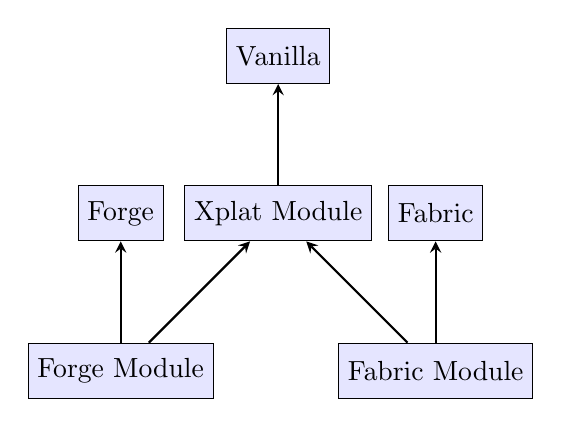
\begin{tikzpicture}[node distance=2cm]
      \node (vanilla) [std] {Vanilla};
      \node (xplat_mod) [std, below of=vanilla] {Xplat Module};
      
      \node (forge) [std, left of=xplat_mod] {Forge};
      \node (fabric) [std, right of=xplat_mod] {Fabric};

      \node (forge_mod) [std, below of=forge] {Forge Module};
      \node (fabric_mod) [std, below of=fabric] {Fabric Module};

      \draw [arrow] (xplat_mod) -- (vanilla);
      \draw [arrow] (forge_mod) -- (xplat_mod);
      \draw [arrow] (forge_mod) -- (forge);
      \draw [arrow] (fabric_mod) -- (xplat_mod);
      \draw [arrow] (fabric_mod) -- (fabric);
    \end{tikzpicture}
  \end{center}
  ``Xplat'' means ``cross-platform''. Darkhax and Jared's example use ``Common'', but that
  is easily confused with common as in ``shared between client and server''.
\end{frame}

\begin{frame}{Downcalls To Platform}
  \begin{center}
    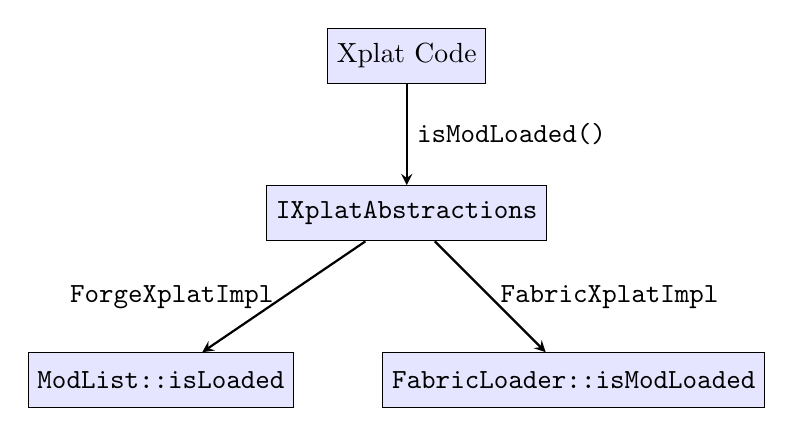
\begin{tikzpicture}[node distance=3cm]
      \node (xplat) [std] {Xplat Code};
      \node (ixplat) [std, node distance = 2cm, below of=xplat] {\texttt{IXplatAbstractions}};
      \node (forge) [std, below left of=ixplat, xshift = -1cm] {\texttt{ModList::isLoaded}};
      \node (fabric) [std, below right of=ixplat] {\texttt{FabricLoader::isModLoaded}};

      \draw [arrow] (xplat) -- node[anchor=west] {\texttt{isModLoaded()}} (ixplat);
      \draw [arrow] (ixplat) -- node[anchor=east] {\texttt{ForgeXplatImpl}} (forge);
      \draw [arrow] (ixplat) -- node[anchor=west] {\texttt{FabricXplatImpl}} (fabric);
    \end{tikzpicture}
  \end{center}
  Event firing, capability/API Lookups, etc. all handled this way.
\end{frame}

\begin{frame}{Migrating to Multiloader}
  Recall key takeaway: Refactor in an environment where you can test each step of the way:
  \begin{itemize}
  \item Create empty ``shell'' Xplat and Forge modules, dump \textbf{working} codebase into Fabric module
  \item Incrementally move pieces to Xplat, compile/test every step of the way
  \item Took a couple months to go from running on Fabric...to running on Fabric. Useless?
  \item No! Now it's super clear what needs to be done for Forge: Implement \texttt{ForgeXplatImpl}, and hook up all the entry points and event handlers.
  \end{itemize}
  
\end{frame}

\section{Current Day}
\begin{frame}{Current State}
  Things are great. Gameplay changes only made once, no merge hell across branches.

  Uniqueness of Botania allowing this to go so smoothly:
  \begin{itemize}
  \item We are feature-complete, thus low-churn
  \item Emphasize staying close to vanilla
  \item Mojmap provides an easy \textit{lingua franca} across platforms
  \item Mixin also a \textit{lingua franca} for hooking vanilla
  \item ``Political'' will from maintainers to make it happen
  \end{itemize}
\end{frame}

\begin{frame}{Interesting Stats}
  Some cool stats comparing the code size of each module.
  Produced by \texttt{tokei} on commit \texttt{595d4940}

  
  \begin{tabular}{|c||c|c|}
    \hline
    Module & Significant Java Lines & Significant JSON Lines \\
    \hline\hline
    Xplat  & 67808 & 137450 \\
    \hline
    Forge  & 4277  & 603 \\
    \hline
    Fabric & 4341  & 745 \\
    \hline
  \end{tabular}

  Over 88\% of code depends only on vanilla!\\
  Platform-specific code is mostly initialization code, registering event handlers,
  and mod integrations (JEI, Curios, EMI, Trinkets, etc.)
\end{frame}

\begin{frame}{Wrap-Up}
  Thanks to the following people:
  \begin{itemize}
  \item Botania Team (Hubry, Alwinfy, myself)
  \item BlameJared, Darkhax et al.
  \item All patrons and vip's who helped test
  \end{itemize}

  Please support the fundraiser to retexture Botania!
  Go to \href{https://botaniamod.net/retexture.html}{botaniamod.net/retexture.html} and visit our booth to learn more.
\end{frame}

\begin{frame}
  \begin{center}
    \Huge Questions
  \end{center}
\end{frame}

\end{document}